\section{B-Link-Tree}\label{section:b-link-tree}

Previous approaches include locking a subtree of highest affected node \cite{samadi1976b}, which, albeit straightforward, reduced concurrency. To alleviate the bottleneck without risking inconsistency, \textit{B-Link-Tree} relaxes the definition of B$^+$Trees. As explained by Graefe \cite{goetz-tech}:

\begin{definition}
  B-Link-Tree is a B$^+$Tree with following properties:
  \begin{enumerate}
    \item Each node $x$ has additional attributes:
          \begin{itemize}
            \item $x.sibling$, a pointer to a right sibling node at the same depth,
            \item $x.highkey$, the upper bound of all keys found in the subtree rooted by $x$ (every key found in $x$ is less then $x.highkey$).
          \end{itemize}
    \item Does not require locks nor latches for reading.
  \end{enumerate}
\end{definition}

\begin{figure}[H]
  \centering
  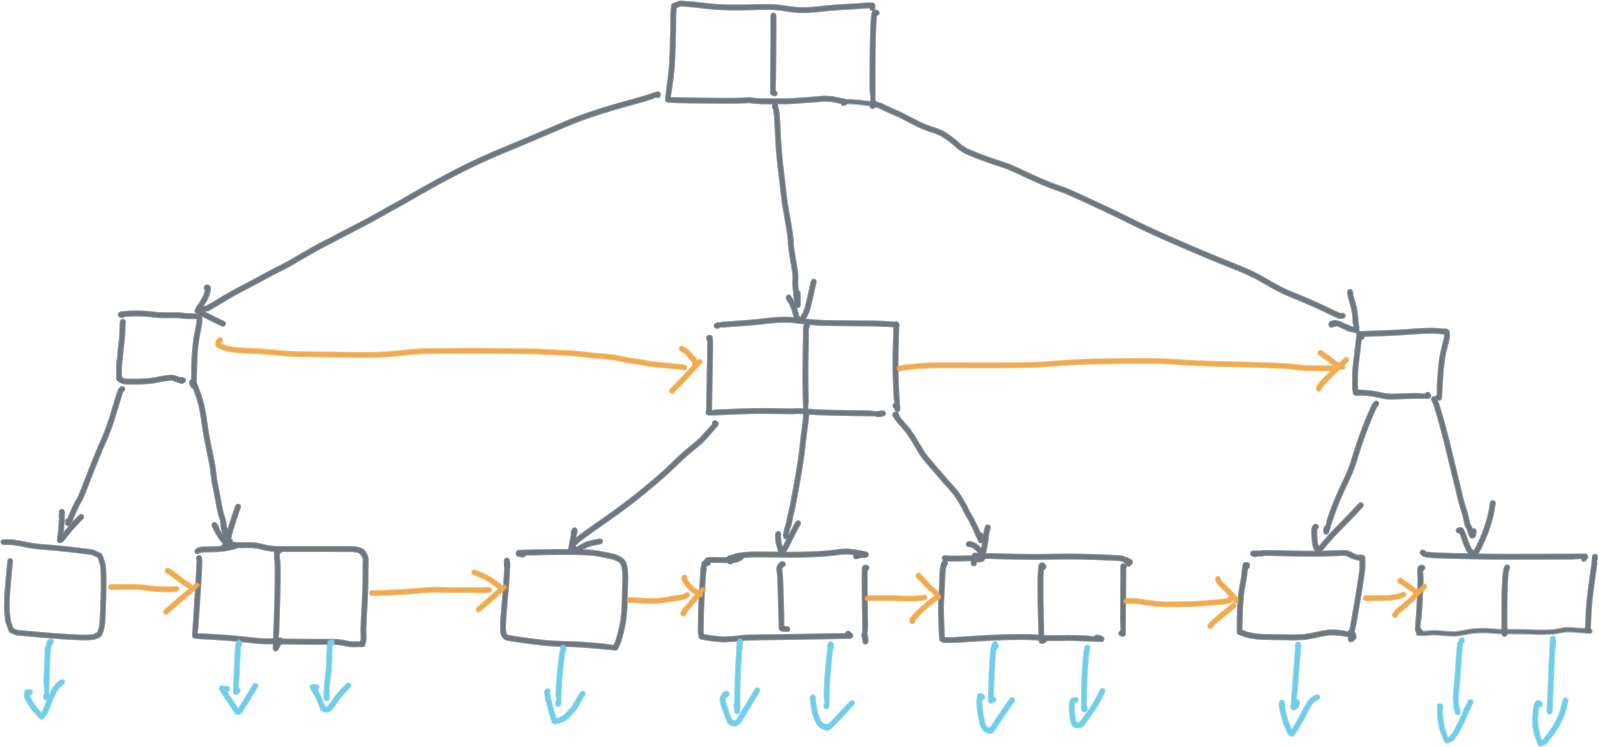
\includegraphics[width=\textwidth]{components/figure/b-link-tree.png}
  \caption{B-Link-Tree with $Order$ = 3}
  \label{figure:b-link-tree}
\end{figure}

Splitting during node insertion is divided into two independent steps: splitting a node and inserting the split node with its new separator key to the parent node. When splitting node $x$, a new right sibling node $y$ is created. The node $y$ inherits the high key from the split node $x$, whereas the first key of $y.keys$ is used as a new $x.highkey$. Thus, an internal node does exist without a parent in between the operations. $x.highkey$ is used to be able to traverse the newly split node and its subtree, even when the split operation is not complete.

\todo{Add insertion pseudocode}

As the final step of node splitting, the separator key and the newly split node $y$ are inserted in the parent node.

\todo{Add search pseudocode}

Tree traversal is modified to honor $x.highkey$ by returning the node at $x.sibling$ when the target key $k$ is larger or equal than $x.highkey$.

\todo{Add interaction correctness proof}

Prove a case of colliding insertion and search operation. We need to consider the case of search operation before insertion is complete (eg: search operation S reads node n insertion operation I modifies the node from n to n', search operation S continues with contents based on n).

Three types of split:
- simple insertion of value/pointer pair
- splitting of a node, insertion to the left (same) node
- splitting of a node, insertion to the right (new) node

Simple insertion into a non-full node. Leaf nodes are trivial, internal nodes inserting a pair. Newly inserted node can be acceseed via the side pointers.

Search while split. If searching in a node mid-split, the search stays the same except for the newly inserted node, which won't be found. If searching in an internal node, \todo{Explain, why nodes below the split node are correct}.

